One of Dr. Jonas' greatest discoveries was the Heyting people, a democratic collection of 6 tribes that lived on the Eurasian steppes.
They kept meticulous records of their elections and their rulers.
Strangely, even though the Heyting people were democratic, the voting records indicated that many of their leaders recived far less than the majority of the votes.
How could this happen?

Well, to simplify the voting process, the tribes had broken their land up into provinces.
Each province had one vote for the next ruler of that tribe, which was based upon
the majority vote from within the province.
However, since the tribe leaders were allowed to redraw the boundaries of the provinces 
each year using the following guidelines,
the minority party was able to keep power.
\begin{enumerate}
\item The number of provinces in each tribe had to stay the same each year.
\item Each province had to be a single connected region.
\item The difference in population between any two provinces had to be 5 or less.
\item All province boundary lines had to follow the horizontal and vertical grid lines provided.
\end{enumerate}

Determine the number of provinces for each Tribe A-E from Dr. Jonas's journal that allowed the minority party
to win the majority of provinces each year. Enter this into ClueKeeper using the format A\#-B\#-C\#-D\#-E\#.
To help, an example is given below.

\begin{center}
Tribe X,
Population = 50,
Provinces = 4

\begin{tabular}{c c c }

Year 1 & Year 2 & Year 3 \\
 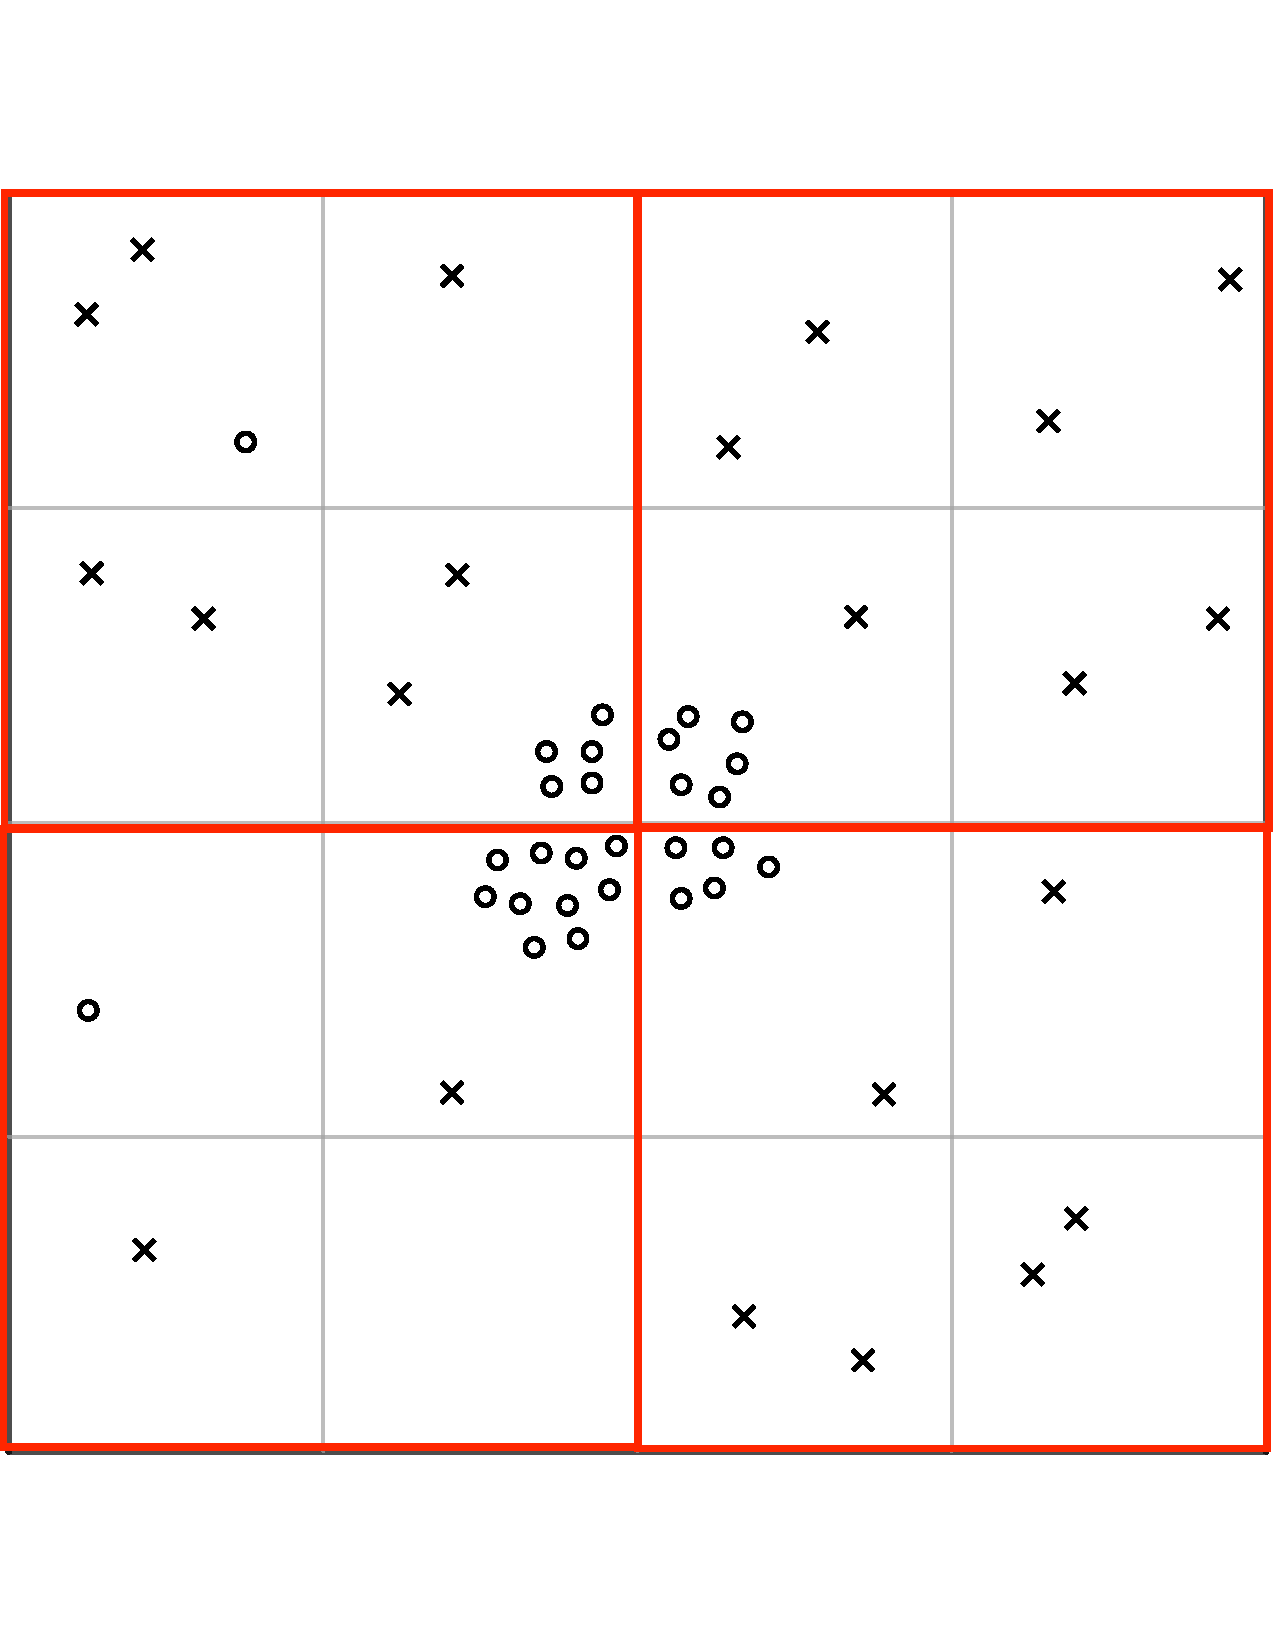
\includegraphics[width=2in]{assets/Gerrymandering/Gerry4x4-50-1Solution.pdf} &  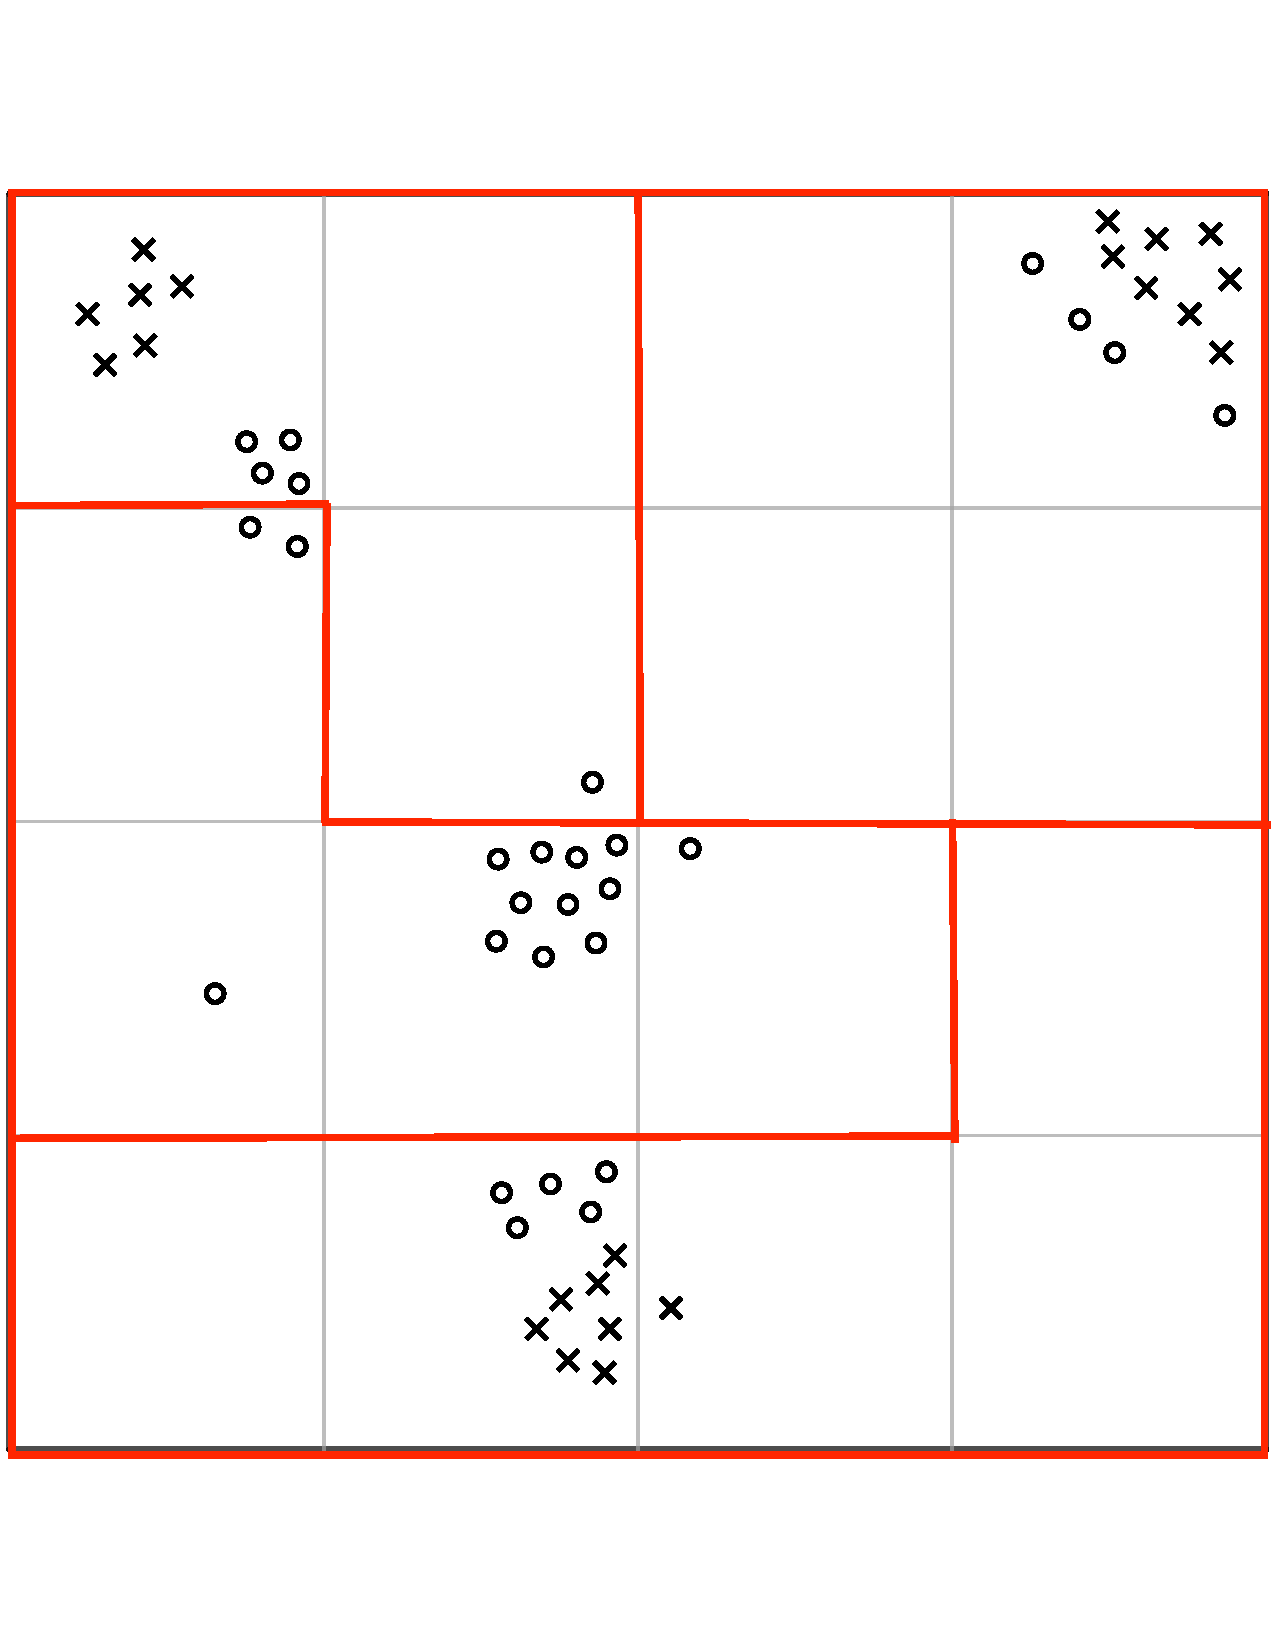
\includegraphics[width=2in]{assets/Gerrymandering/Gerry4x4-50-2Solution.pdf} &  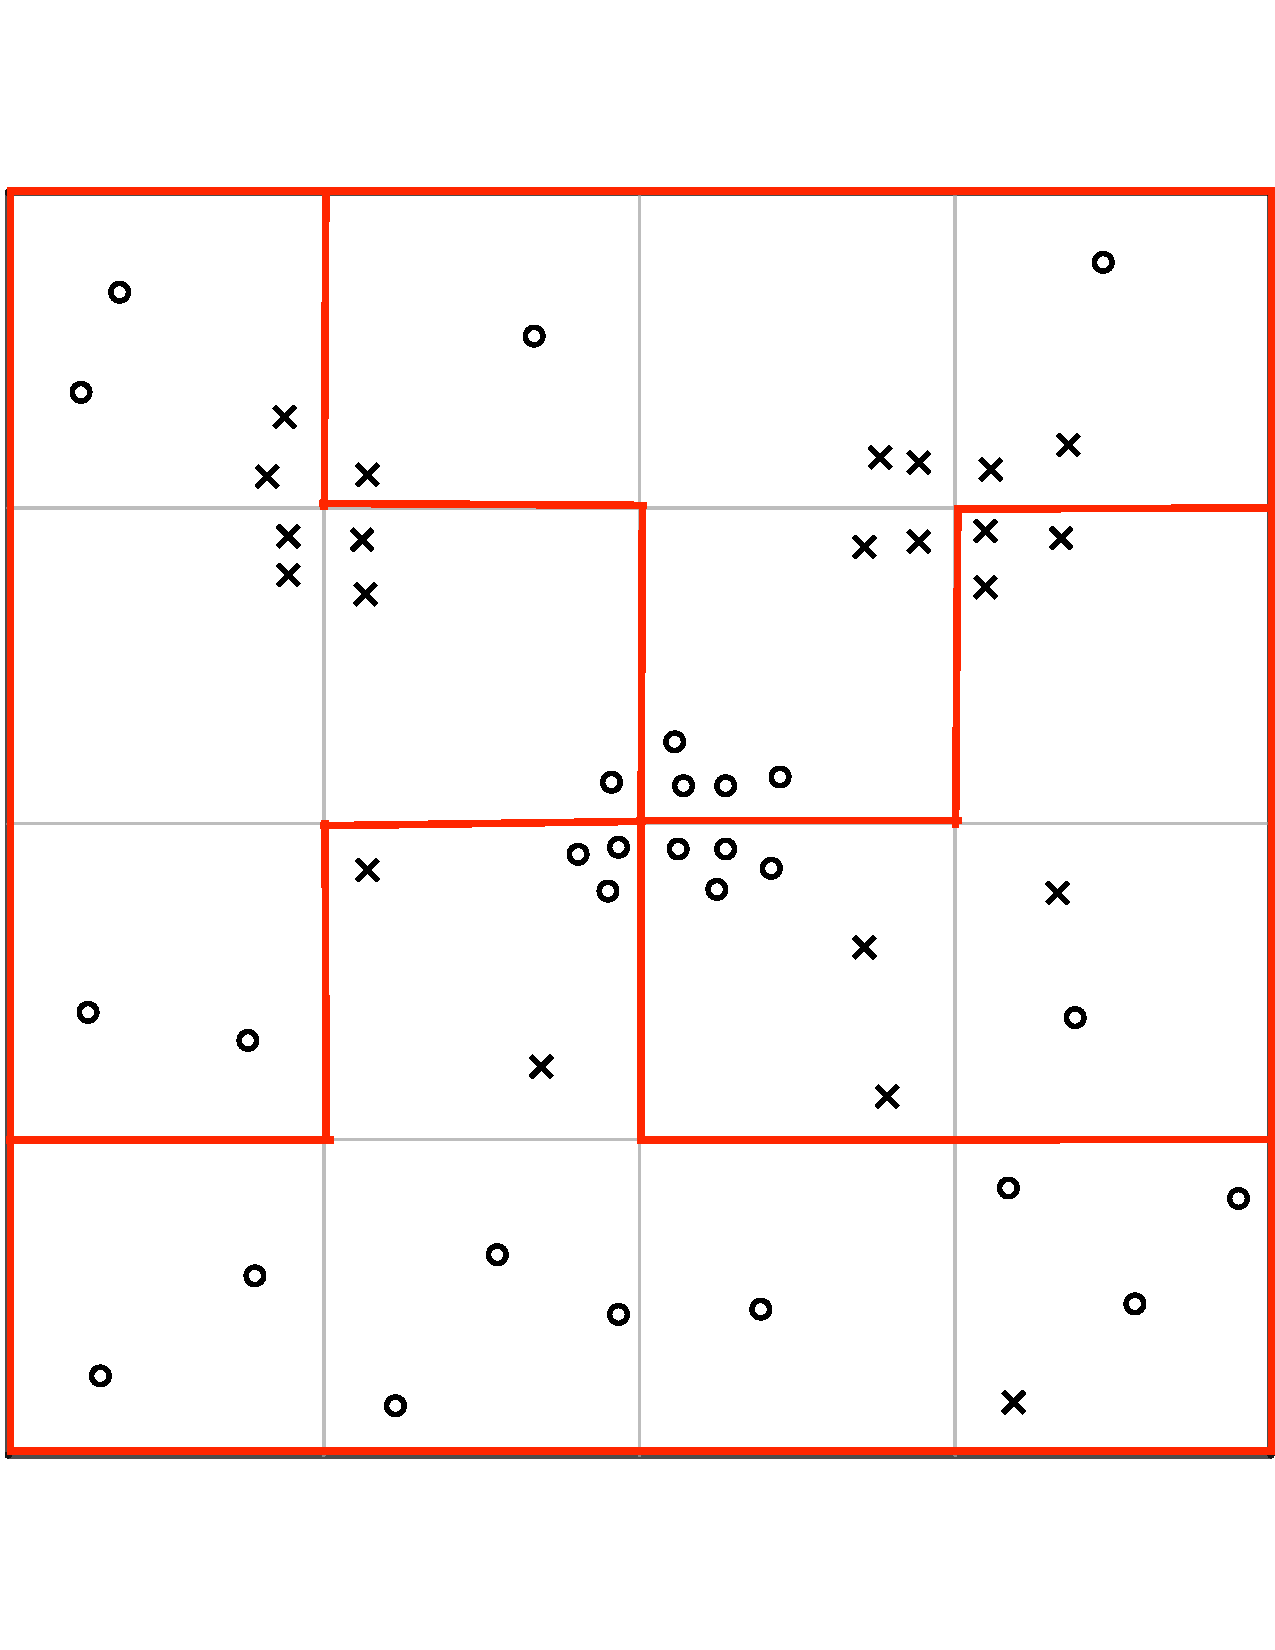
\includegraphics[width=2in]{assets/Gerrymandering/Gerry4x4-50-3Solution.pdf}\\
 Total Vote Count &  Total Vote Count &  Total Vote Count\\
 X - 22 people, \textbf{3 provinces won} & X - 22 people, \textbf{3 provinces won} & X  - 22 people, \textbf{3 provinces won}\\
 O - \textbf{28 people}, 1 province won & O - \textbf{28 people}, 1 province won & O - \textbf{28 people}, 1 province won
\end{tabular}
\end{center}

%Dr. Jonas reasoned that there were 3 provinces for tribe X.
%After finding the number of provinces for the other tribes, you should be able to decode the message in Dr. Jonas' journal.
